\documentclass[3p,times,preprint,number,round]{elsarticle}
%\documentclass[preprint,12pt]{elsarticle}

\newcommand\hmmax{0}
  \newcommand\bmmax{3}
%\usepackage{algorithm2e}
%\usepackage{algorithm}
%\usepackage{algpseudocode}
%\usepackage{algorithmic}
 \usepackage{mathtools}
\usepackage{makeidx}
    \usepackage{float}
    \usepackage{graphicx}
\usepackage{makeidx}  % allows for indexgeneration
\usepackage[english]{babel} % un troisième package
\usepackage{amssymb}
\usepackage{amsmath}
\usepackage{syntax}
\usepackage{multirow}
\usepackage{array}
\usepackage[table]{xcolor}
\usepackage{enumitem}
\usepackage{booktabs}
\usepackage{listings}
\usepackage{verbatim}
%\usepackage{caption}
\usepackage{subcaption}
\usepackage{courier}
%\usepackage{mathrsfs}
%\usepackage[authoryear]{natbib}
%\usepackage{amsthm}
\usepackage{amsthm}
%\usepackage{nath}

\usepackage{lmodern}
%\usepackage{bm}
\usepackage{tikz}
%\usepackage[]{algorithm2e}
%\usepackage{algorithm}


%\usepackage{algorithm}   % For math symbols
%\usepackage[noend]{algpseudocode}
%\usepackage{algorithm2e}
%\usepackage{algorithmic}
\usepackage[ruled,lined,linesnumbered]{algorithm2e}
%\usepackage{algorithm}
%\usepackage{algorithmic}
%\usepackage{algpseudocode}
\usepackage[hyphens]{url}
%\usepackage{breakurl}
%\PassOptionsToPackage{hyphens}{url}
\usepackage{hyperref}
\hypersetup{
  colorlinks,
  citecolor= 	JungleGreen,
  linkcolor= 	JungleGreen,
  urlcolor= 	JungleGreen}
  
  \usepackage{tabularx}
\usepackage{rotating}
\usepackage[T1]{fontenc}
\usepackage[utf8]{inputenc}
%\usepackage{amsmath,amsfonts,amssymb}
%\usepackage{mathastext}
\usepackage[bitstream-charter]{mathdesign}
%\usepackage[T1]{fontenc}
\usepackage{booktabs}
\normalfont
\usepackage{listings}     
\usepackage{lstautogobble}  % Fix relative indenting
\usepackage{color}          % Code coloring
\usepackage{zi4}            % Nice font
\definecolor{bluekeywords}{rgb}{0.13, 0.13, 1}
\definecolor{greencomments}{rgb}{0, 0.5, 0}
\definecolor{redstrings}{rgb}{0.9, 0, 0}
\definecolor{graynumbers}{rgb}{0.5, 0.5, 0.5}
\definecolor{forestgreen}{rgb}{0.0, 0.5, 0.0}

\definecolor{commentgreen}{RGB}{2,112,10}
\definecolor{eminence}{RGB}{108,48,130}
\definecolor{weborange}{RGB}{255,165,0}
\definecolor{frenchplum}{RGB}{129,20,83}

\usepackage[hyphens]{url}
\usepackage{hyperref}
\hypersetup{
  colorlinks,
  citecolor= 	blue,
  linkcolor= 	blue,
  urlcolor= 	blue}
    \usepackage{breakurl}
    
%% set the starting page if not 1
%\firstpage{1}
%%%%%%%%%%%%%%%%%%%%%%%%%%
\DeclareCaptionFont{white}{\color{white}}
\DeclareCaptionFormat{listing}{%
    \colorbox{black}{\parbox{\dimexpr\textwidth-2\fboxsep}{\textbf{\textcolor{white}{#1#2#3}}}}}
\captionsetup[lstlisting]{format=listing,labelfont=white,textfont=white}

%% Give the name of the journal

\usepackage{lineno}

\usepackage{tikz}
\usetikzlibrary{matrix,arrows.meta,arrows,automata,backgrounds}
\tikzset{%
  >={Latex[width=2mm,length=2mm]},
  % Specifications for style of nodes:
            base/.style = {rectangle, rounded corners, draw=black,
                           minimum width=2cm, minimum height=1cm,
                           text centered, font=\sffamily},
  activityStarts/.style = {base, fill=blue!30},
       startstop/.style = {base, fill=red!30},
    activityRuns/.style = {base, fill=green!30},
         process/.style = {base, minimum width=2.5cm, fill=orange!15,
                           font=\ttfamily},
}

\newcommand*\circled[1]{\tikz[baseline=(char.base)]{
    \node[shape=circle, draw, inner sep=1pt, 
        minimum height=12pt] (char) {#1};}}
        \ttfamily

\newcommand{\sensinact}{\texttt{sensi\textbf{N}act}}

\newcommand{\ecircle}[1] {\textcircled{{\small #1}}}


\newcommand{\fig}[1]{Figure \ref{#1}}

\newcommand{\commenting}[1] {\textcolor{red}{#1}}

\newcommand{\quot}[1] {``#1''}

\newcommand{\emath}[1] { $#1$ }

\newcommand{\emathtt}[1] { $\mathtt{#1}$ }

\newcommand{\msym}[1] { $\mathscr{#1}$ }

\newcommand{\alg}[1] {Algorithm \ref{#1}}

\newcommand{\lst}[1] {Listing \ref{#1}}

\newcommand{\ie}{i.e., }
\newcommand{\eg}{e.g., }
\newcommand{\thisrelation}{${\rm I\!R}$}

\newtheorem{theorem}{Theorem}%[section]
\newtheorem{lemma}[theorem]{Lemma}
\newtheorem{proposition}[theorem]{Proposition}
\theoremstyle{definition}
\newtheorem{mydef}{Definition}
\newtheorem{example}{Example}
%\volume{00}
\newcommand{\gparrow}[1] {\lhook\joinrel\xrightarrow{#1} }
%\firstpage{1}
\newcommand{\acisiot} {s\textbf{A}fety and se\textbf{C}ur\textbf{I}ty as\textbf{S}urrance for critical \textbf{IoT} systems}
\journal{Elsevier}

%\newcommand*\circled[1]{\tikz[baseline=(char.base)]{\node[shape=circle,draw,inner sep=2pt] (char) {#1};}}
\usepackage[many]{tcolorbox}  
\usepackage{setspace}               % for LINE SPACING
\usepackage{multicol}               % for MULTICOLUMNS

  
\usetikzlibrary{calc,shadows.blur}
\def\llbracket{[\![}
\def\rrbracket{]\!]}

\newcommand{\sset}[1] {\llbracket #1 \rrbracket}
\newtcolorbox{boxD}{
    colback = gray!5!white, 
    colframe = black, 
    boxrule = 0pt, 
    toprule = 3pt, % top rule weight
    bottomrule = 3pt % bottom rule weight
}

\newtcolorbox{boxC}{
    colback = blue!0!white,  % background color
    boxrule = 0pt  % no borders
}

\newtcolorbox{boxF}{
    colback = yellow!5!white,
    enhanced,
    boxrule = 1.5pt, 
    colframe = white, % making the base for dash line
    borderline = {1.1pt}{0pt}{main, dashed} % add "dashed" for dashed line
}

%\runauth{}
%\jid{procs}
\makeindex

%\jnltitlelogo{\small Information Sciences}
\normalsize

\usepackage{amssymb}

\setcitestyle{square}

\SetSymbolFont{operators}   {normal}{OT1}{cmr} {m}{n}
\SetSymbolFont{letters}     {normal}{OML}{cmm} {m}{it}
\SetSymbolFont{symbols}     {normal}{OMS}{cmsy}{m}{n}
\SetSymbolFont{largesymbols}{normal}{OMX}{cmex}{m}{n}
\SetSymbolFont{operators}   {bold}  {OT1}{cmr} {bx}{n}
\SetSymbolFont{letters}     {bold}  {OML}{cmm} {b}{it}
\SetSymbolFont{symbols}     {bold}  {OMS}{cmsy}{b}{n}
\SetSymbolFont{largesymbols}{bold}  {OMX}{cmex}{m}{n}

\SetMathAlphabet{\mathbf}{normal}{OT1}{cmr}{bx}{n}
\SetMathAlphabet{\mathsf}{normal}{OT1}{cmss}{m}{n}
\SetMathAlphabet{\mathit}{normal}{OT1}{cmr}{m}{it}
\SetMathAlphabet{\mathtt}{normal}{OT1}{cmtt}{m}{n}
\SetMathAlphabet{\mathbf}{bold}  {OT1}{cmr}{bx}{n}
\SetMathAlphabet{\mathsf}{bold}  {OT1}{cmss}{bx}{n}
\SetMathAlphabet{\mathit}{bold}  {OT1}{cmr}{bx}{it}
\SetMathAlphabet{\mathtt}{bold}  {OT1}{cmtt}{m}{n}

\newcommand\myeq{\stackrel{\mathclap{\footnotesize\mbox{def}}}{=}}

\usepackage{enumitem}
%\linenumbers

\newcommand{\eclipse}[1] {\textcolor{eminence}{\texttt{\textbf{#1}}}}

\newcommand{\gtext}[1] {\textcolor{forestgreen}{#1}}

\newcommand{\keyw}[1] {\texttt{\textbf{#1}}}

\newcommand{\gl}[1] {\langle {#1} \rangle}

\newcommand\setItemnumber[1]{\setcounter{enumi}{\numexpr#1-1\relax}}

\newcommand{\cmt}[1] {\textcolor{blue}{#1}}
%%%%%%%%%%%%%%%%%%%%%%%%%%%%%%%%%%%%%%
\usetikzlibrary{calc,shadows.blur}
\tcbuselibrary{skins}
\newtcolorbox{resp}[2][]{%
  enhanced jigsaw,
  colback=gray!20!white,%
  colframe=gray!80!black,
  size=small,
  boxrule=1pt,
  title=#2,
  halign title=flush center,
  coltitle=black,
  drop shadow=black!50!white,
  attach boxed title to top left={xshift=1cm,yshift=-\tcboxedtitleheight/2,yshifttext=-\tcboxedtitleheight/2},
  minipage boxed title=3cm,
  boxed title style={%
    colback=white,
    size=fbox,
    boxrule=1pt,
    boxsep=2pt,
    underlay={%
      \coordinate (dotA) at ($(interior.west) + (-0.5pt,0)$);
      \coordinate (dotB) at ($(interior.east) + (0.5pt,0)$);
      \begin{scope}
        \clip (interior.north west) rectangle ([xshift=3ex]interior.east);
        \filldraw [white, blur shadow={shadow opacity=60, shadow yshift=-.75ex}, rounded corners=2pt] (interior.north west) rectangle (interior.south east);
      \end{scope}
      \begin{scope}[gray!80!black]
        \fill (dotA) circle (2pt);
        \fill (dotB) circle (2pt);
      \end{scope}
    },
  },
  #1,
}


\begin{document}

\begin{frontmatter}

%\dochead{}
%Formalizing the Detection and Mitigation of Clock Deviation in Challenging Physical and Environmental Conditions for Synchronous and Asynchronous Communication Styles

%\title{Security Risk Assessment of the RabbitMQ Protocol through Concurrent Stochastic Games}
%\title{Security Risk Assessment of the RabbitMQ Broker using Concurrent Stochastic Games}

%\title{\cmt{Rigorous Analysis of Learned Attack Patterns in RabbitMQ Broker with Concurrent Stochastic Games}}

\title{\cmt{Rigorous Security Analysis of RabbitMQ Broker with Concurrent Stochastic Games}}

% \author[aut2]{Abdelhakim Baouya\corref{cor1}}
% \ead{abdelhakim.baouya@gmail.com}

% \author[aut2]{Brahim Hamid}
% \ead{brahim.hamid@irit.fr}

% \author[aut4]{Levent Gürgen}
% \ead{levent@kentyou.com}

% \author[aut3]{Saddek Bensalem}
% \ead{saddek.bensalem@univ-grenoble-alpes.fr}

% \cortext[cor1]{Corresponding author at : University of Toulouse, IRIT, France}


% \address[aut2]{University of Toulouse, IRIT, France}

% \address[aut3]{Université Grenoble Alpes, VERIMAG, Grenoble, France}

% \address[aut4]{Kentyou Company, France}

\begin{abstract}
Modern Internet of Things architectures encompass \cmt{various} computational logic and communication protocols. However, the security issues inherent in these systems pose significant risks, \cmt{especially at the device edges}. Addressing security threats on the \cmt{deployed communication edges} is imperative to ensure a robust and secure communication system. In this study, we propose an approach that utilizes the Concurrent Stochastic Game model (CSG) to specify the behavior of RabbitMQ \cmt{Broker} in the context of IoT systems precisely while considering potential data corruption attacks. For parametrizable evaluation, these attacks and their frequencies are learned. We implement the CSG model in \cmt{PRISM games} for automated analysis, leveraging reward Probabilistic Alternating Temporal Logic (rPATL) to model security requirements as game goals. Empirical validation of the work is presented via an industrial case study that shows how \cmt{data} corruption attacks can impact the sensed data in water dam infrastructure. \cmt{This assessment gives valuable insights into the RabbitMQ deployment at the edge.} 

%To validate our approach, we investigate data corruption attacks targeting sensed data and examine its impact on payload routing and message loss for water dam infrastructure. 
\end{abstract}

\begin{keyword}
Edge computing\sep Game Model\sep Security Threats \sep Formal methods.
\end{keyword}
\end{frontmatter}

\tableofcontents

\newpage

\section{Introduction}

\begin{sloppypar}

Edge computing is a paradigm that decentralizes computational power, bringing it closer to the point of data generation, such as IoT devices (\cmt{sensors and actuators}). Unlike relying on a centralized cloud infrastructure, edge computing focuses on processing and analyzing data at or near the network edge, where it originates \cite{KHAN2019219}. However, \cmt{security} concerns have become significant in modern IoT systems \cite{baouya2022}. Insecure network connections pose risks such as data interception, unauthorized access, and tampering \cite{Hossein2023}. Hence, it is of utmost importance to identify and address these security concerns during the early stages of development \cite{Valentina2024, Brahim2018}. This underscores establishing precise semantic definitions for threats and attacks at the design phase.


To develop new and innovative Edge Servers with specific functionalities, enterprise companies rely on (mainly open source) \quot{middleware} software \cite{ZHANG2021}, which needs to be enhanced with custom software components to implement multiple functions, including security, that add value compared to other edge servers on the market. Notably, middlewares have been tailored to process signals efficiently and route them from IoT sensors to nodes employing application-level protocols like Hypertext Transfer Protocol Secure (HTTPS) \cite{Prasenjit2019}. Beyond that, the literature shows recent advancements in developing appropriate protocols for \cmt{ edge core-side infrastructures (e.g., AMQP\footnote{\url{https://www.amqp.org/}}) facilitating device-edge communication (e.g., CoAP~\cite{coap})}. 

Among the wide range of \cmt{brokers} available, RabbitMQ\footnote{\url{https://www.rabbitmq.com/}} stands out as a message queue middleware that facilitates asynchronous message communication. It leverages the capabilities of the Erlang language \cite{armstrong2013programming} to implement the Advanced Message Queuing Protocol (AMQP) adopted by reputable vendors such as JPMorgan, NASA, Red Hat, Google, IBM, VMware, Mozilla, and others.
In this paper, we undertake a comprehensive analysis of the security of RabbitMQ architecture using formal methods. We employ the model checker PRISM-games to formalize and verify RabbitMQ as a Concurrent Stochastic Game (CSG)\cite{kwiatkowskaautomatic2021}, leveraging reward Probabilistic Alternating Temporal Logic (rPATL) \cite{hutchisonautomatic2012} to model security \cmt{properties} as game goals. To validate our work, we explore a set of potential attacks at two distinct levels of the protocol:  \emph{messages received} and \emph{queues}.   


\subsection{Contributions} 
To the best of our knowledge, RabbitMQ has not been examined for potential attacks within the context of a CSG formalism.  In the available literature, the research conducted by \cite{Li2020} primarily centers around examining functional properties employing UPPAAL \cite{behrmann2006uppaal}. Contrarily, studies conducted by \cite{Ionescu2015,Hong2018,Bagaskara2020,Rostanski2014}  primarily utilize simulation techniques to assess performance aspects pertaining to the deployed servers, encompassing scalability, memory usage, and throughput. Nevertheless, these studies do not incorporate the modeling of attacks within the system. The paper under consideration contributes significantly to the field by addressing this gap, with the main contributions summarized as follows:

\begin{enumerate}
    \item Formalizing RabbitMQ to comprehensively understand its communication \cmt{broker} behavior using operational semantics rules.

    \item Formalizing the CAPEC-384 attack scenario using operational semantics rules.
    
    \item Developing an interpretation of the formal representation of RabbitMQ under attacks in the formalism of PRISM-games.
    
    \item Examining attacks in a use case scenario that addresses the deployment of RabbitMQ on a communication gateway.

    
\end{enumerate}

By employing formal methods for studying attacks within the system, we provide valuable insights that enhance the understanding of the system's security aspects. The paper uses a set of abbreviations and references in Table \ref{tableOfacronyms}.

%Presently, within enterprise companies, there is a multitude of open-source middleware that have gained significant adoption. One noteworthy firm in this domain is Kentyou\footnote{\url{http://kentyou.com/}}, which has flourished as a result of successful European and international projects. Kentyou's notable accomplishment includes the development of the Sensinact gateway, which exhibits the seamless translation of messages between various protocols. Notably, it has been tailored to process efficiently and route signals from IoT sensors to nodes employing application-level protocols like HTTPS. Moreover, the edge infrastructure encompasses a wide range of existing open-source protocols, including MQTT and CoAP (see deliverables \cite{sensinactref2024}).



%To bolster the capabilities of the Sensinact gateway on the edge server, we undertake a comprehensive analysis of the RabbitMQ architecture utilizing formal methods. To accomplish this, we employ the model checker PRISM-games to formalize and verify RabbitMQ as a Concurrent Stochastic Game (CSG)\cite{kwiatkowskaautomatic2021}. Our research specifically targets potential attacks, including DoS (Denial of Service) and ARP Spoofing, at two distinct levels of the protocol: messages received and queues. 



\begin{table}[h!]
\centering

\begin{tabular}{|m{1.50cm} l |} 
\hline 
ATL & Alternating Temporal Logic \\
ARP & Address Resolution Protocol \\
CAPEC & Common Attack Pattern Enumeration and Classification \\
DDoS &  Distributed Denial of Service \\
CTL & Computation Tree Logic \\
CSG & Concurrent Stochastic Game \\
ILP & Integer Linear Programming \\
MC & Model Checking \\
MDP & Markov Decision Process \\
MITM & Man in the Middle \\
PCTL & Probabilistic Computation Tree Logic \\
rPATL & reward Probabilistic Alternating Temporal Logic \\
SMC & Statistical Model Checking \\
WL & Water Level \\
WV & Water Volume \\ 
RP & Rain Precipitation \\ 
\hline 
\end{tabular}
\caption{A List of Acronyms Used in the Article.}
\label{tableOfacronyms}
\end{table}
\normalsize

\subsection{Outline} 


The subsequent sections of this paper are organized as follows: In Section \ref{Preliminaries}, we \cmt{provide} preliminaries encompassing the Concurrent Stochastic Game (CSG) and PRISM-games language. Following that, in Section \ref{Approach}, we present the workflow of the study. Section \ref{frequencies} presents the flow for learning attack frequencies. In Section \ref{rabbitmq}, we employ CSG to model RabbitMQ and address security concerns. In Section \ref{sec:useCase}, we conduct an experiment within the context of IoT systems for the practical application of our approach. In Section \ref{discussion}, an extensive discussion is presented, covering potential enhancements in scalability and outlining strategies for mitigating attacks. Section \ref{sec:rw} \cmt{summarizes} the related works, highlighting their contributions and limitations. Lastly, in Section \ref{conclusion}, we conclude our work by \cmt{outlining} the key findings and proposing directions for future research.

\end{sloppypar}

\section{Background}
\label{Preliminaries}
\begin{sloppypar}
This section covers the essential concepts related to Concurrent Stochastic Multi-player Games and their implementation in PRISM games. \cmt{Furthermore, We will revisit the AMQP protocol stack, which is essential for understanding message routing.}

\subsection{Concurrent Stochastic  Games}
Concurrent stochastic games (CSGs) \cite{kwiatkowskaautomatic2021, fismancorrelated2022} consider that players make choices concurrently in each state and then transition simultaneously. In CSGs, players have control over one or more modules, and the actions associated with these modules can only be utilized by the respective player who owns them. The CSG is defined as an extension of Probabilistic Automata (PA) \cite{ref27} in \cite{kwiatkowskaautomatic2021, fismancorrelated2022} as follows:

%This makes CSGs distinct from approaches to automata synchronization based on common action labels. 

\begin{mydef} \label{def:csg} \normalfont A concurrent stochastic multi-player game (CSG) is a tuple \emath{G =\gl{s_{0}, S, N, A, \Delta, \delta, AP, L}}:

\begin{itemize}
	\item \emath{s_{0}} is an initial state, such that \emath{s_{0} \in S},
	\item \emath{S} is a set of states,
	\item \emath{N =\{1,...,n\}} is a finite set of players,
	 \item \emath{A= \Sigma_{1} \times \ldots \times \Sigma_{n} } where \emath{\Sigma_{i}} is a finite set of actions available to player \emath{i \in N},
     \item \emath{\Delta: S \longrightarrow 2^{\cup_{i=0}^{n} \Sigma_{i}}} is an action assignment function,
 
    \item \emath{\delta : S \times A \longrightarrow Dist(S)} is a probabilistic transition function assigning for each \emath{s \in S} and \emath{(\alpha_{0},\ldots, \alpha_{n}) \in \Sigma_{i} } a probabilistic distribution \emath{\mu \in Dist(S)}, and \emath{L: S \longrightarrow 2^{AP}} is a labeling function that assigns each state  \emath{s \in S}  to a set of atomic propositions taken from the set of atomic propositions (\emath{AP}).
\end{itemize}
\end{mydef}


When in state s, each player \emath{i \in N} selects an action from its available actions \emath{Action_{i}(s) \myeq \Delta(s) \cap \Sigma_{i}} if this set is non-empty.  A path \emath{\pi} of a CSG \emath{G} \cite{kwiatkowskaautomatic2021, fismancorrelated2022} is a sequence \emath{\pi = s_{0}\xrightarrow{\alpha_{i}}s_{1}} where \emath{s_{i} \in S}, \emath{\alpha_{i} = (a_{j}^{1}, . . . , a_{j}^{n}) \in A}, \emath{\alpha_{i}^{j} \in Action_{i} (s_{i})} for \emath{i \in N} and \emath{\delta(s_{j}, \alpha_{j})(s_{j+1}) > 0} for all \emath{j > 0}. 


CSGs are augmented with reward structures \cite{kwiatkowskaautomatic2021}  as \emath{r_{A} : S \times A \longrightarrow \mathbb{R}} is an action reward function that assigns a real value to each pair of state and action tuples, which accumulates when the action tuple is selected in the corresponding state and \emath{r_{s} : S \longrightarrow \mathbb{R}}  is a state reward function assigns a real value to each state, which accumulates when the state is reached.


The properties related to CSGs are expressed in the temporal logic rPATL \cite{hutchisonautomatic2012} (reward Probabilistic Alternating Temporal Logic). The property grammar is based on CTL \cite{baierprinciples2008} extended with coalition operator \emathtt{\langle\langle C\rangle\rangle} of ATL \cite{Alur2002} and probabilistic operator \emathtt{P} of PCTL \cite{hanssonlogic1994}. For instance, for the following property expressed in natural language: \quot{\emph{Players 1 and 2 have a strategy to ensure that the probability of shutdown occurring within 100 steps is less than 0.001, regardless of the strategies of other players}} is expressed in rPATL as: \emathtt{\langle\langle 1,2\rangle\rangle P_{<0.001} [ F^{\leq100} shutdown].} Here, \quot{\emathtt{shutdown}} is the label that refers to the system states. Concerning rewards structure, the property expressed in natural language: \quot{\emph{What is the maximum commutative reward r within 100 steps to reach \quot{\emathtt{fail}} for both Players 1 and 2 for a selected strategy ?}} is expressed  in rPATL as \emathtt{\langle\langle 1,2\rangle\rangle R _{max=?} [ C^{\leq 100}] }

\begin{example}
\label{exp:csg:architecture}   
Consider the CSG shown in \fig{fig:even:odds}, which corresponds to two players repeatedly performing a scheduled read and write operation. Transitions are labeled with actions where \emath{A = (r_{1}r_{2}), (w_{1}w_{2}), (w_{2}r_{1}), (r_{2}w_{2}), (reset_{1} reset_{2})}. The CSG starts in state 's0', and states 's1', 's2', and 's3' are labeled with atomic propositions corresponding to a player winning. Each player communicates through writing and reading operations.
%\tikzset{every picture/.style={ scale=0.95,line width=0.2pt}} %set default line width to     
\noindent
\begin{figure}[!htb]
    \centering
  \includegraphics[width=250pt, height =200pt]{examplecsg.pdf}
    \caption{Read and Write Game Model in CSG.}
    \label{fig:even:odds}
\end{figure} 

In relation to the modeled system, if Player 1 commences the game and that player emerges victorious as it performs writing, the property is expressed as \emathtt{\langle\langle 1,2 \rangle\rangle P_{>0.99}=? [ F \ win=1 ]}. The model and properties associated with the example are available at \cite{edcc23}. 

\end{example}
%\end{paperexample}

\subsection{The PRISM-games language}
We rely on the CSG model to express the coalition game in PRISM language \cite{Kwiatkowskaprism2011}. The PRISM model is composed of a set of modules that can synchronize. A set of variables and commands characterizes each module. The variable's valuations represent the state of the module. A set of commands is used to describe the behavior of each module (i.e., transitions). A command takes the form: \emath{ [a_{j}, \ldots, a_{m}] g \rightarrow \lambda_{1}: u_{1} + \ldots+ \lambda_{n}: u_{n} } or, \emath{[a_{j}, \ldots, a_{m}] g \rightarrow u}, which means, for actions \quot{\emath{a}} if the guard \quot{\emath{g}} is true, then, an update \quot{\emath{u_{i}}} is enabled with a probability \quot{\emath{\lambda_{i}}}. A guard is a logical proposition consisting of variable evaluation and propositional logic operators. The update \quot{\emath{u_{i}}} is an evaluation of variables expressed as a conjunction of assignments: \emath{v_{i}'=val_{i}+\ldots+v_{n}'=val_{n}} where \quot{\emath{v_{i}}} are local variables and \emath{val_{i}} are values evaluated via expressions denoted by \quot{\emath{eval}} such that \emath{ eval: V \rightarrow \mathbb{D}}.
Let \emath{\mathbb{D}} be a domain of variables such as \emath{\mathbb{D}=\mathbb{N} \cup \{true,false\} }. We define valuations for variables as \quot{\emath{\theta}} such that \emath{ \theta: V \rightarrow \mathbb{D} } that associate each variable in \emath{V} with a value in \emath{\mathbb{D}}. We use \emath{l_{0}, l_{1},\ldots, l_{n}} as new valuations of variables \emath{v_{0}, v_{1},\ldots, v_{n}}. Each PRISM command is encapsulated within a PRISM module \cite{KWIATKOWSKA20065} defined as follows:

\begin{mydef} \label{def:prismmodule} \normalfont (PRISM-Module). A PRISM module \quot{\emath{\mathcal{D}}} is a tuple \emath{\mathcal{D}= \langle \vartheta_{L}, Cm\rangle}, where: 
 \begin{itemize}
\item \emath{\vartheta_{L}} is a finite set of local variables associated with the module \emath{\mathcal{D}} initialized with \emath{init},
\item \emath{Cm} is a finite set of commands that defines the behavior of module \emath{\mathcal{D}}. Formally, we consider the command of the form \emath{ [a_{0}, \ldots, a_{m}] g \rightarrow \lambda: u} as \emath{l_{i}\xrightarrow{g:\gl{ a_{j}, \ldots, a_{m}}}_{\lambda}l'_{i}} such that \emath{l_{i}\models g}, \emath{g \in Const(V)} and \emath{\theta':=\theta[v_{i}:=eval(v_{i})]}.
            \end{itemize}
\end{mydef}

\begin{example}
In the PRISM code of \lst{exampleinprism}, a dedicated non-player module  is used for orchestrating read and write operations. All commands are labeled with at least two ports, which correspond to the players responsible for triggering the internal write and read operations. The "win" variable defines the player's success in writing (taking values 1 or 2).
The first commands shown in lines 5-6 represent unscheduled writing (i.e., reading) operations. As these operations are executed, a reset command is introduced in line 8 to indicate an idle state. Subsequently, the commands depicted in lines 9-10 enforce an order between writing and reading operations.  The model and properties associated with the example are available at \cite{edcc23}.

\lstdefinestyle{framed}
{
	frame=lrb,         
	mathescape,
	numbers=left,
	belowcaptionskip=-1pt,
    xleftmargin=3em,
		xrightmargin=0.01cm,
    framexleftmargin=3em,
	framexrightmargin=0pt,
	framextopmargin=5pt,
	framexbottommargin=5pt,
	framesep=0pt,
	rulesep=0pt,
	numbers=left,
}
    
\lstset{
    breaklines=true,
    style=framed,
    escapeinside={<@}{@>},
    morekeywords={void, int, public, private, class, protected, submodules, network, connections, const, init, int, bool, double, module, rewards, endrewards, endmodule},
    basicstyle=\ttfamily,
    keywordstyle=\bfseries\color{blue},
        morecomment=[f][\color{green!30!black}][0]{/*},
    morecomment=[l][\color{green!30!black}]{//},
    label=queueemodel
}



\begin{figure}[!htb]            
\begin{minipage}{15.5cm}
\begin{lstlisting}[style=framed,%customc,
	caption=PRISM Code for Read/Write of \fig{fig:even:odds},
 	label=exampleinprism]	
module recorder // a non player model in charge of recording players actions
 win : [0..2]init 0;
 a : [0..2]init 0;
	
 [w1,w2] s=0 -> (s'=1) & (win'=0);
 [r1,r2] s=0 -> (s'=1) & (win'=0);

 [reset1,reset2] s=1 | s=2 | s=3 -> (s'=0) & (win'=0);
 [r1,w2] s=0 -> (s'=2) & (win'=2);
 [w1,r2] s=0 -> (s'=3) & (win'=1);
endmodule
\end{lstlisting}
 \end{minipage}  
\end{figure}

\end{example}

\subsection{The RabbitMQ broker}
\cmt{RabbitMQ, a message broker, implements the Advanced Message Queuing Protocol (AMQP), standardized in ISO/IEC 19464:2014 \cite{ISOAMQP}. AMQP defines the communication rules for messages where RabbitMQ serves as a concrete implementation. This paper utilizes the AMQP 0.9/1.0 implementation provided by RabbitMQ \cite{Rabbitmq}. The reference communication stack, depicted in \fig{fig:rabbitmq:arch}, is adapted from the AMQP Architecture specification (AMQP Architecture:  \cite{Rabbitmq} and \cite{amqp-architecture}). (1) Application Layer: This layer interacts with applications using client libraries and defines a message format and semantics (\emph{see section 2.1 AMQ Model Architecture} in  \cite{Rabbitmq}). (2) Messaging Layer: This layer handles message routing, exchanges, queues, and bindings (\emph{see section 3.1.1 Messages and Content} in \cite{Rabbitmq}), with a focus on message routing and distribution. (3) Framing Layer: This layer takes messages from the messaging layer and packages them into frames with specific headers and content data (\emph{see section 2.3.5 Frame Details} in  \cite{Rabbitmq}), focusing on data structuring and encapsulation. (4) Transport Layer: This layer provides reliable and secure communication between peers (RabbitMQ clients/servers). It typically uses TLS/SSL for encryption and TCP for reliable delivery (\emph{many features are discussed in section 2.3 AMQP Transport Architecture} in  \cite{Rabbitmq}). (5) Wire Level: This layer defines the byte format on the network for each frame (\emph{see section 4.2 AMQP Wire-Level Format} in \cite{Rabbitmq}), addressing low-level network communication details.}

\noindent
\begin{figure}[!htb]
    \centering
  \includegraphics[width=170pt, height =190pt]{architecture.pdf}
    \caption{RabbitMQ Implementation of AMQP Architecture\cite{amqp-architecture}.}
    \label{fig:rabbitmq:arch}
\end{figure} 

The main feature that can justify the use of the RabbitMQ broker for IoT implementing AMQP and in the case of IoT gateway \cite{sensinactref2024, Baouyasaddek2024} is \cmt{the implementation of a CoAP-to-RabbitMQ. It can bridge the communication gap between resource-constrained devices and robust messaging systems. This bridge translates CoAP messages into the richer format used by RabbitMQ. This approach fosters interoperability, allowing diverse device types to participate in a unified communication ecosystem supported by gateways in \cite{sensinactref2024}. In addition, RabbitMQ broker implements clustering functions \cite{rabbitmq-clustering} that enhance the availability and reliability of the infrastructure.}



\end{sloppypar}

\section{Approach}
\label{Approach}
\begin{sloppypar}
This paper implements the workflow depicted in \fig{workflow} for modeling the RabbitMQ \cmt{broker} and conducting security analysis. 

\begin{figure}[h]
\noindent
     \centering
		\includegraphics[width=470pt, height =150pt]{flow.pdf}
		\caption{A Workflow for Learning, Modeling, and Verification of the RabbitMQ \cmt{Broker}}
	\label{workflow}
\end{figure}



% Learning step : 
\paragraph{Frequencies learning} The frequencies of attacks, such as DoS, Mirai, and ARP spoofing, have been learned \cmt{from} a collected dataset using the algorithm described in Section \ref{frequencies}. These attack frequencies are required for populating the PRISM model.

\paragraph{Modeling} The modeling phase entails translating protocol specifications, described in natural language \cite{Rabbitmq}, into a PRISM model consisting of modules that adhere to the PRISM language (as discussed in Section \ref{Preliminaries}). This process results in a parametrizable PRISM model. Our work enhances this process by incorporating security considerations and formalizing specific attack scenarios within the CSG PRISM-supported language. The attack scenario examined in this research focuses on CAPEC-384 \cite{capec384}, which involves the \quot{\emph{Application API Message Manipulation via Man-in-the-Middle}}. Therefore, the parametrizable PRISM model is populated with attack frequencies to capture the stochastic nature of the attacks within their cyber-physical environment. These frequencies represent the occurrence of attacks as probabilistic phenomena derived from an Open-Source dataset. 

\paragraph{Probabilistic model checking} To assess the potential risks inherent in the RabbitMQ \cmt{broker} regarding attacks, we utilize rPATL properties. The risk involves assessing the likelihood of an attack occurring and its potential consequences on the communication protocol \cite{Grzegorz2011}. The rPATL properties provide an indication of the degree of data corruption in the \cmt{form} of game goals resulting from manipulated data within the \cmt{broker} using the PRISM-games model checker. By considering these properties, we gain insights into risks that may arise within the RabbitMQ \cmt{broker}. 






\end{sloppypar}

\section{Learning Attack Frequencies}
\label{frequencies}
\begin{sloppypar}
This section delves into the process of learning attack frequencies from \cmt{input dataset}. We assume attacks occur within specific timeframes, as illustrated in \fig{attacks}. The Mean Time Between Attacks (MTBA) is extracted from the dataset using established algorithms like the Broyden–Fletcher–Goldfarb–Shanno (L-BFGS-B) algorithm described in \cite{liu1989limited} and the Nelder-Mead algorithm \cite{nelder1965simplex}. \cmt{Section~\ref{sec:rw} will discuss additional algorithms inspired by natural behaviors \cite{Genghis2023, Ezugwu2022, Jeffrey2022, Agushaka2023, Mojtaba2024, DETDO2023} that can be employed for this purpose.}



\begin{figure}[h]
\noindent
     \centering
		\includegraphics[width=300pt, height =100pt]{timeline.pdf}
		\caption{Mean Time Between Attacks}
	\label{attacks}
\end{figure}



%The L-BFGS algorithm is widely employed for optimizing problems involving large datasets. On the other hand, the Nelder-Mead algorithm, also known as the downhill simplex method, constructs a geometric shape in the parameter space to search for the optimal solution efficiently. 

The classical approach for calculating the mean time involves considering the initial attack detected along with its successors, divided by the total number of attacks in the dataset. Formally, for a dataset consisting of \emath{n} features: \emath{f_{1},\ldots, f_{n} \in F}  where each feature is associated with its domain \emath{ Dom: F \rightarrow \mathbb{D}}. \emath{\mathbb{T}} is the time domain for attack feature occurrence. We are able to implement the Algorithm \ref{algo:attacks}. The algorithm is a simple exploration of the dataset where two attacks are collected \emath{a_{1}} and \emath{a_{2}}, where \emath{a_{2}} is the successor of \emath{a_{1}}. When an attack is detected, its successor is determined and the difference is stored in the stack. Subsequently, the mean time between attacks is calculated once the successor is empty. For handling large datasets, we utilize both the L-BFGS and Nelder-Mead algorithms. The Python source code for this implementation can be found in the Artefacts section \ref{sub:artefact}.

\RestyleAlgo{ruled}

%% This is needed if you want to add comments in
%% your algorithm with \Comment
\SetKwComment{Comment}{\gtext{/*} }{ \gtext{*/}}
\begin{algorithm}[H]
\label{algo:attacks}
\caption{Mean Time Between Attacks Computation. }
%\caption{An algorithm with caption}\label{alg:two}
\KwData{Feature \emath{f_{i}.}}
\KwResult{p as attack frequency.}
$Stack \gets Empty$ \Comment*[r]{\gtext{A stack of meantime of attacks.}}
$a_{1} \in \mathbb{T}$ \Comment*[r]{\gtext{initial attacks.}}
$a_{2} \in \mathbb{T}$ \Comment*[r]{\gtext{sucessor of the attack.}}
 
\For{ line \emath{\in} dataset }{ 
     \If{attack \emath{\in} line}    {
            $a_{1} = extractTimefrom feature(f_{i}, attack)$ \Comment*[r]{\gtext{Extract the first attack.}}
            
            $a_{2} = extractNextAttackTimefromfeature(f_{i}, attack)$\Comment*[r]{\gtext{Extract the successor of the first attack.}}
            
            $Stack.append(|a_{2}-a_{1}|)$\Comment*[r]{\gtext{Store the time differences}}
        }
        
     \If{$a_{2}$ is $Empty$}    {
            $satisfy \gets false$;

            $p \gets meanTime(Stack)$ \Comment*[r]{\gtext{Store the calculated mean time as the probability of an attack occurring.}}
        }

             

}
\end{algorithm}

\end{sloppypar}


\section{RabbitMQ architecture and threats modeling}
\label{rabbitmq}
\begin{sloppypar}

% \subsection{The Sensinact edge gateway}
% The communication between sensors/actuators and the Edge is facilitated by a gateway. An edge gateway, also referred to as an edge device, is a network device that functions as the entry point for data traffic between diverse networks. In addition to routing and protocol conversion, the edge gateway fulfills various functions. It plays a crucial role in enabling the seamless data flow between networks while ensuring connectivity and interoperability. Typically, the edge gateway is deployed at the network's edge, serving mainly as protocol conversion. In the work context, we depend on the Sensinact gateway, which has been brought to fruition after a series of European projects, namely BigClouT \cite{ref144}, WISE IoT \cite{ref145}, IoF2020 \cite{ref146}, ActivAge \cite{ref147}, and ultimately Brain-IoT \cite{brainiot2022}. The specificity of the Sensinact gateway lies in its ability to enable designers and edge architects to specify the data flow using the Sensinact language. The \fig{sensinact} portrays the internal structure of the Sensinact gateway composed of northbound and southbound bridges. The \textit{northbound} bridge provides crucial functionalities for interfacing with remote servers using costly protocols such as HTTP/HTTPS. It supports a wide range of protocols, such as HTTP REST, MQTT, XMPP, JSON RPC, and CDMI.  The \textit{southbound} module facilitates the interaction with sensors and actuators, utilizing various device protocols such as Zigbee, LoRa, and MQTT. In this paper, we will not address the details related to the gateway as they are available in the Brain-IoT deliverables. We would to enhance the southbound bridges of the gateway by supporting RabbiotMQ protocol \cite{Rabbitmq}. The difference from southbound bridge protocols, such as MQTT, lies in its support for asynchronous messages through  message queuing.


This section presents the formalization of the RabbitMQ Architecture to make it compatible with the Concurrent Stochastic Game (CSG). We also provide a formal implementation of RabbitMQ in PRISM games. We formalize and model the CAPEC-384 \cite{capec384} attack at various protocol levels, specifically focusing on data corruption, and establish semantic rules to capture their impact.



\subsection{The RabbitMQ architecture}
%In \fig{rabbitarchitecture}, we illustrate the architecture of RabbitMQ, which consists of a set of sensors (Producers) and one actuator (consumer). A Raspberry Pi serves as a connectivity interface that converts signals into data sensitive to attacks and acts as both a consumer and producer. The exchange is responsible for accepting messages from the producers and routing them to message queues based on \textbf{binding key}. For example, the water level queue is associated with the binding key \emph{binding key = wl\_pl}. The exchange examines the message properties derived from the sensor's message to extract the \textbf{routing key}, a virtual address used to determine which message queue the message will be stored in by matching the binding keys. 

%\BH{Update the figure with the FOG and the Gateway explicitley}

In \fig{fig:rabbitarchitecture}, we present the architectural depiction of RabbitMQ deployed on an IoT gateway. This deployment comprises a set of Producers, specifically three sensors: water level (WL), water volume (WV), and rain precipitation (RP), as well as two consumers, including one actuator and the Fog. Additionally, a connectivity interface is incorporated to convert signals into data, which is susceptible to attacks, and it serves both the consumers and producers. The exchange is designed to accept messages from the producers and direct them to message queues based on a designated \textbf{binding key}. For instance, the water level queue is associated with the binding key \emph{binding key = wl\_pl}. The exchange scrutinizes the message properties derived from the producers' messages in order to extract the \textbf{routing key}, which functions as a virtual address that determines the appropriate message queue for storage by matching the binding keys. Formally, a RabbitMQ system during execution is defined as follows:

\begin{mydef} \label{def:rq} \normalfont (RabbitMQ). A RabbitMQ system \quot{\emath{\mathcal{RQ}}} is a tuple \emath{\mathcal{RQ}= \langle \mathcal{M}, RK, BK, E, Q\rangle}, where: 
 \begin{itemize}
\item \emath{\mathcal{M}} is the message structure alive in \emath{\mathcal{RQ}}, 
\item \emath{RK}= \emath{\{ rk_{0}, \ldots,rk_{n} \} } is a set of routing keys,
\item \emath{BK}= \emath{ \{ bk_{0}, \ldots,bk_{n}  \} } is a set of binding keys,
\item \emath{E} is the exchange node of the system, and 
\item \emath{Q} = \emath{\{ q_{0}, \ldots, q_{n}\}} is a set of queues supported by \emath{\mathcal{RQ}}. 
            \end{itemize}
\end{mydef}


Throughout the paper, we consider a message composed of a \emph{routing key and a payload}. Formally, we define a RabbitMQ message as:

\begin{mydef} \label{def:message} \normalfont (Message). A RabbitMQ message \quot{\emath{\mathcal{M}}} is a tuple \emath{\mathcal{M}= \langle rk, pld\rangle}, where: 
 \begin{itemize}
\item \emath{rk} is the routing key of sensors message and
\item \emath{pld} is the payload of the sensed data
            \end{itemize}
\end{mydef}
\begin{figure}[!htb]
           
\noindent
     \centering

		\includegraphics[width=263pt, height =200pt]{ArchitectureRabbit.pdf}
		\caption{The RabbitMQ Architecture for IoT.}
	\label{fig:rabbitarchitecture}
\end{figure}

\subsection{Communication formalism for RabbitMQ architecture in PRISM-games}
%\BH{missing D3!!}
In the PRISM-games formalism, the modeling of communication and resource access is facilitated through the use of player and non-player modules. Players are distinguished by unique action labels, while non-CSG players are identified by multiple action labels. For instance, each component of the modeled system in \fig{fig:rabbitarchitecture} is considered as a PRISM module where reading and writing is enabled by access to local PRISM module variables.


%In the PRISM module, \emath{rk} and \emath{pld} are local variables initialized to queue keys and sensed data, respectively. Each component of the modeled system in \fig{fig:rabbitarchitecture} is considered as a PRISM module where reading is enabled to other PRISM models with the PRISM system.


The algebraic expression of the message \emath{m} transmitted from module \emath{\mathcal{D}_{1}} to \emath{\mathcal{D}_{2}} is expressed through channeling \cite{baierprinciples2008} using send (!) and receive (?) symbols as : \emath{\sset{\mathcal{D}_{s}}=l_{1} \gparrow{\langle a!m \rangle} l_{2}} saying that  \emath{\mathcal{D}_{s}} transmit the message through the channel \emath{a} (PRISM action) and \emath{\sset{\mathcal{D}_{r}}=l_{3} \gparrow{\langle a?x \rangle}l_{4}} saying that \emath{a?x} receives a message via channel \emath{a} and assign it to variable \emath{x}.


However, building upon the player definition provided in the previous section, we introduce a two-player rule that involves a competition based on writing. \emath{\mathcal{D}_{3}} records the messages received from both players \emath{\mathcal{D}_{1}} and \emath{\mathcal{D}_{2}.}The rule \ref{writing} is defined as follows:

\begin{boxD}
%\framedtext{
	      \begin{equation}\frac{\sset{\mathcal{D}_{1}}= l_{1}\gparrow{a!m_{1}}l'_{1} \wedge \sset{\mathcal{D}_{2}}= l_{2}\gparrow{b!m_{2} }l'_{2}  \wedge
        \sset{\mathcal{D}_{3}}= l_{3}\gparrow{a?k_{1}, b?k_{2}}l'_{3}        
       } {  \langle l_{1},\ldots,l_{2},\ldots l_{3},\theta\rangle  \xrightarrow{a,b}\langle l'_{1},\ldots,l'_{2},\ldots,l'_{3},\theta'\rangle } \tag{\emph{Writing}} \label{writing} \end{equation} where \emath{\theta':=\theta[ k_{1}:= m_{1}, k_2:=m_{2}]} and \emath{\mathcal{D}_{1}, \mathcal{D}_{2}} are two CSG players.
%}

\end{boxD}


\subsection{Queues modeling}
\label{sec:threats:manif}

The RabbitMQ queues are responsible for storing the sensed data based on the routing key present in the transmitted messages. The Exchange module verifies the correspondence between the routing key and the binding key in order to carry out the operation. Firstly, the \emath{Queue} module is regarded as a player responsible for data storage. It is characterized by the queue variable and the identifier binding key, as depicted in lines 1-3 of the code snippet of \lst{queueemodel}. As the PRISM language lacks native support for the list data type, it is necessary to define the list cases and the index variable, as mentioned in lines 1-2. To traverse the queue, we require an item index that is initialized to 0 at line 5. 
\noindent
\begin{figure}[!htb]
    \centering
    \input{queuelatex.tex}
    \caption{Queue Model.}
    \label{fig:queue}
\end{figure} 

To enhance clarity, the enqueue and dequeue operations are modeled as automata in \fig{fig:queue}. At each state (corresponding to an index value), the \emph{enqueue} operation is performed, and the variables \emath{b_{0},\ldots,b_{1}} are assigned the value of the payload, denoted as $pld$ following the rule \ref{writing}. The consumer (for example a Fog) executes the dequeue operation, while a non-player module stores the dequeued data that will be consumed. The command in line 6 executes the automata model depicted in \fig{fig:queue}, where each state represents an index value. Additionally, we utilize a conditional structure in command line 6 to assign the value of $pld$ to the corresponding variable $b_{i}$ based on the index value. In the dequeue operation, the synchronization based on the dequeue channel is carried out with the command in line 9.

\lstdefinestyle{framed}
{
	frame=lrb,         
	mathescape,
	numbers=left,
	belowcaptionskip=-1pt,
    xleftmargin=3em,
		xrightmargin=0.01cm,
    framexleftmargin=3em,
	framexrightmargin=0pt,
	framextopmargin=5pt,
	framexbottommargin=5pt,
	framesep=0pt,
	rulesep=0pt,
	numbers=left,
}
    
\lstset{
    breaklines=true,
    style=framed,
    escapeinside={<@}{@>},
    morekeywords={void, int, public, private, class, protected, submodules, network, connections, const, init, int, bool, double, module, rewards, endrewards, endmodule},
    basicstyle=\ttfamily,
    keywordstyle=\bfseries\color{blue},
        morecomment=[f][\color{green!30!black}][0]{/*},
    morecomment=[l][\color{green!30!black}]{//},
    label=queueemodel
}



\begin{figure}[!htb]            
\begin{minipage}{16cm}
\begin{lstlisting}[style=framed,%customc,
	caption=PRISM Code for the Queue Player,
 	label=queueemodel]	
module Queue
 $b_{0}$: [INIT_VAL..MAX_VAL]  init EMPTY;
 $b_{1}$: [INIT_VAL..MAX_VAL]  init EMPTY;
 $bk$ : [KEY_0..KEY_0] init KEY_0;
 i   :[0..QUEUE_MAX] init 0;
 [enqueue] i<QUEUE_MAX -> (i'=mod(i+1,QUEUE_MAX))  &($b_{0}$'=(i=0)?$pld_{3}$:$b_{0}$) &($b_{1}$'=(i=1)?$pld_{3}$:$b_{1}$);
 [dequeue] i>0 -> (i'=i-1)  &($b_{0}$'=(i=0)?EMPTY:$b_{0}$)  &($b_{1}$'=(i=1)?EMPTY:$b_{1}$); 
endmodule
\end{lstlisting}
 \end{minipage}  
\end{figure}

The model, consisting of one producer (sensor), one queue, and one consumer (fog), can be accessed through the following link: \cite{edcc23} under reference \texttt{M2}. In the following section, we instantiate multiple queues and sensors to facilitate the exchange of messages through a use case.



\subsection{Attacks modeling}
\label{sec:threats:manif}

In this section, we formalize the attack CAPEC-384 \cite{capec384} that can impact the messages exchanged between communicating entities, thereby affecting both the payload and the routing key. For each message $m$ we use the following notations:  $rk$ denotes the routing key of the message $m$, $rk_{x}$ denotes the erroneous routing key of the message $m$, $pld$ denotes the payload of the message $m$, and $pld_{x}$ denotes the erroneous payload of the message $m$.

\emph{Tampering} \cite{shostack2014threat}  leads to the alteration of messages transmitted by the sender component through the communication port. Within the context of \emath{\mathcal{RQ}} system, ${pld}$ is altered during the message transfer. Considering the sensor player \emath{\mathcal{D}_{1}} and attacker player \emath{\mathcal{D}_{2}} where the exchange node manages the interaction modeled as \emath{\mathcal{D}_{3}}. When refining the rule (\ref{writing}), the outcomes of routing key tampering are expressed through rules \ref{rkSuccess} and \ref{rkFailure}. Specifically, rule \ref{rkSuccess} represents the successful tampering of the routing key, while rule \ref{rkFailure} represents the failure to tamper with the routing key.

%\BH{refer in the text to \emph{rk Success} and \emph{rk Failure}}

\begin{boxD}
%\framedtext{
	      \begin{equation}\label{rkSuccess} \frac{ \sset{\mathcal{D}_{1}}= l_{1}\gparrow{a!\gl{rk_{1},pld_{1}}}l'_{1} \wedge \sset{\mathcal{D}_{2}}= l_{2}\gparrow{b!\gl{rk_{x},pld_{2}} }l'_{2} \wedge
         \sset{\mathcal{D}_{3}}= l_{3}\gparrow{a, b?\gl{rk_{3},pld_{3}}}_{p}l'_{3}       
       } {  \langle l_{1},\ldots,l_{2},\ldots l_{3},\theta\rangle  \xrightarrow{a,b}_{p}\langle l'_{1},\ldots,l'_{2},\ldots,l'_{3},\theta'\rangle } \tag{\emph{rk Success}} \end{equation} where \emath{\theta':=\theta[rk_{3}=rk_{x},pld_{3}=pld_{2}]} and \emath{\mathcal{D}_{1}} is the sensor, \emath{\mathcal{D}_{2}} is the attacker. \emath{p} is the success rate of the attacker.

	      \begin{equation}\label{rkFailure}\frac{ \sset{\mathcal{D}_{1}}= l_{1}\gparrow{a!\gl{rk_{1},pld_{1}}}l'_{1} \wedge \sset{\mathcal{D}_{2}}=  l_{2}\gparrow{b!\gl{rk_{x},pld_{2}} }l'_{2} \wedge
         \sset{\mathcal{D}_{3}}= l_{3}\gparrow{a, b?\gl{rk_{3},pld_{3}}}_{1-p}l'_{3}       
       } {  \langle l_{1},\ldots,l_{2},\ldots l_{3},\theta\rangle  \xrightarrow{a,b}_{1-p}\langle l'_{1},\ldots,l'_{2},\ldots,l'_{3},\theta'\rangle } \tag{\emph{rk Failure}} \end{equation} where \emath{\theta':=\theta[rk_{3}=rk_{1},pld_{3}=pld_{1}]} and \emath{\mathcal{D}_{1}} is the sensor, \emath{\mathcal{D}_{2}} is the attacker. \emath{1-p} is the failure rate of the attacker.
\end{boxD}


Since the model incorporates the stochastic behavior of the system, it accurately represents the success and failure of the attacker using a stochastic parameter \emath{p}. 

% Add a reference to the learning frequencies algorithm presented in section ***

This parameter enables us to effectively model the message loss of the sensor at the exchange level as a result of the attack. While we address the issue of routing key tampering, it is also necessary to model payload tampering caused by similar attacks. Then, the success and failure rules are expressed by the rules \ref{pld Success} and \ref{pld Failure}.


\begin{boxD}
%\framedtext{
	      \begin{equation}\frac{ \sset{\mathcal{D}_{1}}= l_{1}\gparrow{a!\gl{rk_{1},pld_{1}}}l'_{1} \wedge \sset{\mathcal{D}_{2}}=  l_{2}\gparrow{b!\gl{rk_{2},pld_{x}} }l'_{2} \wedge
        \sset{\mathcal{D}_{3}}=  l_{3}\gparrow{a, b?\gl{rk_{3},pld_{3}}}_{p}l'_{3}      
       } {  \langle l_{1},\ldots,l_{2},\ldots l_{3},\theta\rangle  \xrightarrow{a,b}_{p}\langle l'_{1},\ldots,l'_{2},\ldots,l'_{3},\theta'\rangle } \label{pld Success} \tag{\emph{pld Success}} \end{equation} where \emath{\theta':=\theta[rk_{3}=rk_{1},pld_{3}=pld_{x}]} and \emath{\mathcal{D}_{1}} is the sensor, \emath{\mathcal{D}_{2}} is the attacker. \emath{p} is the success rate of the attacker.
%}
	      \begin{equation}\frac{\sset{\mathcal{D}_{1}}= l_{1}\gparrow{a!\gl{rk_{1},pld_{1}}}l'_{1} \wedge \sset{\mathcal{D}_{2}}= l_{2}\gparrow{b!\gl{rk_{2},pld_{x}} }l'_{2} \wedge
        \sset{\mathcal{D}_{3}}=  l_{3}\gparrow{a, b?\gl{rk_{3},pld_{3}}}_{1-p}l'_{3}       
       } {  \langle l_{1},\ldots,l_{2},\ldots l_{3},\theta\rangle  \xrightarrow{a,b}_{1-p}\langle l'_{1},\ldots,l'_{2},\ldots,l'_{3},\theta'\rangle } \label{pld Failure}  \tag{\emph{pld Failure}} \end{equation} where \emath{\theta':=\theta[rk_{3}=rk_{1},pld_{3}=pld_{1}]} and \emath{\mathcal{D}_{1}} is the sensor, \emath{\mathcal{D}_{2}} is the attacker. \emath{1-p} is the failure rate of the attacker.
\end{boxD}

Now, with the formal specification of attacks at the exchange, we can proceed to provide a projection onto the PRISM code. Before modeling the exchange module of the interaction system, we present in \fig{fig:attack:sensor} the attacker and producer players model. They are characterized by two channels (we employ the terminology used for the channeling system \cite{baierprinciples2008}): write and wait. The write channel is responsible for transmitting the produced value from the producer (i.e., attacker) to the exchange node. The writing and waiting operations are performed each round \emath{r}. 

\noindent
\begin{figure}[!htb]
    \centering
    \input{attackersensormodel}
    \caption{Attacker and Sensor Models.}
    \label{fig:attack:sensor}
\end{figure} 


The exchange system captures the interactions between producers (sensors) and attackers in the \lst{exchangemodel}, specifically focusing on the payload transfer. This is achieved through the utilization of two channels, namely $write_{1}$ and $write_{2}$. The success and failure rules, denoted as \ref{pld Success} and \ref{pld Failure}, are implemented through the PRISM commands found in lines 4-5. Additionally, players have the ability to enter a waiting mode, which is modeled using two channels, $wait_{1}$ and $wait_{2}$, implemented as actions in PRISM. In the case of waiting modes, the exchange module resets both internal binding keys and payload in line 6. However, if one of the players is available to transfer its payload, a non-probabilistic command is implemented in lines 7-8.

\lstdefinestyle{framed}
{
	frame=lrb,         
	mathescape,
	numbers=left,
	belowcaptionskip=-1pt,
    xleftmargin=3em,
		xrightmargin=0.01cm,
    framexleftmargin=3em,
	framexrightmargin=0pt,
	framextopmargin=5pt,
	framexbottommargin=5pt,
	framesep=0pt,
	rulesep=0pt,
	numbers=left,
}
\lstset{
    breaklines=true,
    style=framed,
    escapeinside={<@}{@>},
    morekeywords={void, int, public, private, class, protected, submodules, network, connections, const, init, int, bool, double, module, rewards, endrewards, endmodule},
    basicstyle=\ttfamily,
    keywordstyle=\bfseries\color{blue},
        morecomment=[f][\color{green!30!black}][0]{/*},
    morecomment=[l][\color{green!30!black}]{//},
    label=queueemodel
}



\begin{figure}[!htb]            
\begin{minipage}{16.5cm}
\begin{lstlisting}[style=framed,%customc,
	caption=PRISM code for Exchange Module,
 	label=exchangemodel]	
module Exchange
$pld_{3}$  : [INIT_VAL..MAX_VAL] init EMPTY;
$rk_{3}$ : [INIT_VAL..MAX_VAL] init EMPTY;
[$write_{1}$, $write_{2}$] true  -> (1-$p$):($pld_{3}$'=$pld_{1}$)&($rk_{3}$'=$rk_{3}$)  +$p$:($pld_{3}$'=$pld_{2}$)&($rk_{3}$'=$rk_{2}$);
[$wait_{1}$ , $wait_{2}$]  true -> ($pld_{3}$'=EMPTY) & ($rk_{3}$'=EMPTY);
[$write_{1}$, $wait_{2}$ ]  true -> ($pld_{3}$'=$pld_{1}$) &  ($rk_{3}$'=$rk_{1}$ );
[$wait_{1}$ , $write_{2}$]  true -> ($pld_{3}$'=$pld_{x}$) &  ($rk_{3}$'=$rk_{2}$ );
endmodule
\end{lstlisting}
 \end{minipage}  
\end{figure}

\paragraph*{Remark}The definition of binding key tampering follows the same principle as payload tampering.


\end{sloppypar}



\section{Experiments}\label{useCase}
\label{sec:useCase}
\begin{sloppypar}
%The use case scenario is based on a previously published paper in the \emph{Journal of Applied Intelligence} \cite{baouyageneration2022} for smart water flow assessment. The industrial case study involves the Cecebre dam infrastructure located in Spain. The primary objective of this dam is to collect water from the Meirama Lake and store it in the Cecebre Reservoir from the city of La Coruña; this reservoir plays a vital role in meeting water supply demands for various purposes. Three sensor nodes gather and transmit diverse measurements such as water level (WL), water volume (WV), and rain precipitation (RP) payload to the Fog system to assess the water flow (WF). The internal digital architecture of the industrial use case is partially depicted in \fig{rabbitarchitecture}. The deployment of RabbitMQ on the Sensinact gateway has not yet been completed. As a result, questions regarding the feasibility of this deployment are being addressed and explored in our study. We aim to gain a deeper understanding of potential attack impact. 

In the context of our experiments, we refer to a use case scenario from the collaborative European research project~\cite{brainiot2022} for smart water flow assessment. Three sensor nodes gather and transmit diverse measurements such as water level (WL), water volume (WV), and rain precipitation (RP) payload to the Fog system through 
the Sensinact gateway~\cite{sensinactref2024} to assess the water flow (WF). The internal digital architecture of the industrial use case is partially depicted in \fig{fig:rabbitarchitecture}. 
The deployment of RabbitMQ on the Sensinact gateway has not yet been completed. As a result, questions regarding the feasibility of this deployment are being addressed and explored in our study. 
We aim to gain a deeper understanding of the potential impact of an attack.  

% In the context of our experiment, we used the algorithm (ref) to compute the attacks freqnecices and used them as a parameter for CSG models.... 

The requirements described below are a summary (with some revisited information) of the security properties of RabbitMQ. They are expressed as a set of properties in natural language to protect the corresponding assets.
\begin{boxF}
\begin{itemize}
    \item \emph{\bfseries{Property 1}}: When the sensors transmit payload messages ($wv$, $wl$, and $rp$ $\in [1\ldots3]$) to the fog, we are interested in determining the probability of payload tampering at each round.
    \item \emph{\bfseries{Property 2}}: When the sensors transmit payload ($wv$, $wl$, and $rp$ $\in [1\ldots3]$) messages to the fog, our objective is to determine the probability of message loss after each round.
    \item \emph{\bfseries{Property 3}}: When the sensors transmit payload ($wv$, $wl$, and $rp$ $\in [1\ldots3]$) messages to the fog, Our objective is to determine the probability of message loss caused by the unrouted payload after each round (Tampering affecting only routing keys).
\end{itemize}
\end{boxF}
We intend to provide a formal specification of the functional and security requirements for message delivery that RabbitMQ must fulfill to ensure its effectiveness. We will consider DoS, MITM ARP spoofing, and Mirai attacks at southbound bridges (sensors) and queues. 


\subsection{\cmt{Experimental setup}}
\cmt{Our analyses rely on PRISM-games v4.7, where experiments are conducted on an Ubuntu-I7 system with 32GB RAM. The system model is accessible via the link provided in \cite{edcc23} and adheres to the \emph{CSG} formalism supported by PRISM-games. The engine is set to \quot{Explicit}; other engines are supported by PRISM that offers performance regarding model structure (Please refer to documentation). Player definitions within the model are identified by \quot{player tag} delimiters. For example, the player \texttt{p1} represents the attacker, as exemplified in: \texttt{player p1  Attacker endplayer}. Parameters associated with data manipulation attacks are derived from the dataset denoted as \quot{\texttt{C1}} in \cite{edcc23}. The selection of attack frequency hinges on the chosen scenario, declared as a \texttt{const int} variable. For instance, scenario 1 corresponds to DDoS attacks, scenario 2 to ARP attacks, and scenario 3 to Mirai attacks. A dedicated Python code was developed to calculate the attack rate based on this dataset. Properties relative to our models are expressed in the Modeling section.}


% \cmt{For our analyses, we utilized PRISM-games v4.7, where all experiments were performed on an Ubuntu-I7 system equipped with 32GB of RAM. The system model used in our study can be accessed via the provided link \cite{edcc23}. The PRISM model is \texttt{CSG} supported by PRISM-games. The Engine deleted is \quot{Explicit}. The players definitions in the model are expressed between player tag definition. for instance the player \texttt{p1} refers to the attacker in : \texttt{player p1  Attacker endplayer}. Parameters associated with attacks involving data modification were obtained from the dataset referenced as \quot{\texttt{C1}} in \cite{edcc23}. The selection of the attack frequency is based on the selected scenario (declared as \texttt{const int} ), for instance secanri takes 1 for DDoS 2 for ARP and 3 for Mirai attacks. A Python code was developed to calculate the attack rate based on this dataset}.

\subsection{Modeling}
\label{prop:validation}
%We intend to provide an informal overview of the functional and security requirements for message delivery that RabbitMQ must fulfill to ensure its effectiveness. In our analyses, we utilized PRISM-games v4.7. All experiments were conducted on an Ubuntu-I7 system with 32GB of RAM. The modeled system is available at the link: \cite{edcc23} with reference \texttt{M3}. Parameters related to attacks involving data modification were collected from the dataset provided in \cite{edcc23} under reference \texttt{C1}. A Python code was developed to compute the attack rate using this dataset. 

The RabbitMQ models are partitioned into two distinct models to analyze the impacts of threats on different components of the architecture, specifically the southbound bridges (\quot{M3}) and queues (\quot{M4}). This division is essential to address the challenges of the state space explosion.



We enhance the model by incorporating an integer constant as in \cite{KNPS19} and a module (see \lst{lst:rounds}) to keep track of the number of rounds. In this case, as the commands are unaffected by the players' choices, they are considered unlabelled with empty action. Consequently, these commands are executed regardless of the actions taken by the players. Furthermore, the module is deterministic due to the disjoint guards present in both commands.
\lstset{
    breaklines=true,
    style=framed,
    escapeinside={<@}{@>},
    morekeywords={void, int, public, private, class, protected, submodules, network, connections, const, init, int, bool, double, module, rewards, endrewards, endmodule},
    basicstyle=\ttfamily,
    keywordstyle=\bfseries\color{blue},
        morecomment=[f][\color{green!30!black}][0]{/*},
    morecomment=[l][\color{green!30!black}]{//},
    label=queueemodel
}

\begin{figure}[!htb]            
\begin{minipage}{16.5cm}
\begin{lstlisting}[style=framed,%customc, 
caption=Rounds module to Express multiple Tentatives ,
 	label=lst:rounds]	
const k; // number of rounds
module rounds // module to count the rounds
 rounds : [0..k+1];
 [] rounds<=k -> (rounds'=rounds+1);
 [] rounds=k+1 -> true;
endmodule
\end{lstlisting}
 \end{minipage}  
\end{figure}




\cmt{The properties are defined as a set of requirements in rPATL, mapped from the original natural language expressions in the use case}.

%\emph{\bfseries{REQ1}}: When the sensors transmit payload messages ($wv$, $wl$, and $rp$ $\in [1\ldots3]$) to the fog, we are interested in determining the probability of payload tampering at each round.

 
	    
	    \begin{resp}{\textbf{\textit{Property 1}}}
        \begin{equation}
        \label{eq1}
        \mathtt{\gl{\gl{\textcolor{red}{p1},\textcolor{red}{p2}}}Pmax=? [ !\quot{\textcolor{red}{payload\_tamper}} U \quot{\textcolor{red}{payload\_tamper}}  ]}, \mathtt{\ \textcolor{red}{rounds}=\textcolor{blue}{1}:\textcolor{blue}{30}:\textcolor{blue}{1}} 
        \end{equation}
        \end{resp}
       
        
% \emph{\bfseries{REQ2}}: When the sensors transmit payload ($wv$, $wl$, and $rp$ $\in [1\ldots3]$) messages to the fog, our objective is to determine the probability of message loss after each round.
 
	   
	    \begin{resp}{\textbf{\textit{Property 2}}}
        \begin{equation}
        \label{eq2}
        \splitdfrac{\mathtt{ \gl{\gl{\textcolor{red}{p1}}}R{\{\quot{\textcolor{red}{damage}}\}}max=? [ F \ \textcolor{red}{r}=\textcolor{red}{rounds} ]/}}{\mathtt{\ \gl{\gl{\textcolor{red}{p2}}}R{ \{\quot{\textcolor{red}{sent}}\}}max=? [ F\ \textcolor{red}{r}=\textcolor{red}{rounds} ],  \ \textcolor{red}{rounds}=\textcolor{blue}{1}:\textcolor{blue}{30}:\textcolor{blue}{1}}}
        \end{equation}
        \end{resp}
        

In the context of reward structure, \quot{damage} refers to intercepted and corrupted messages, while total messages \quot{sent} by sensors represent the overall number of messages transmitted.
        
% \emph{\bfseries{REQ3}}: When the sensors transmit payload ($wv$, $wl$, and $rp$ $\in [1\ldots3]$) messages to the fog, Our objective is to determine the probability of message loss caused by the unrouted payload after each round (Tampering affecting only routing keys).
 
	   
	    \begin{resp}{\textbf{\textit{Property 3}}}
        \begin{equation}
        \label{eq3}
        \splitdfrac{\mathtt{ \gl{\gl{\textcolor{red}{p1},\ldots,\textcolor{red}{p8}}}R{\{\quot{\textcolor{red}{empty}}\}}max=? [ F \ \textcolor{red}{r}=\textcolor{red}{rounds} ]/}}{\mathtt{\ \gl{\gl{\textcolor{red}{p1},\ldots,\textcolor{red}{p8}}}R{ \{\quot{\textcolor{red}{sent}}\}}max=? [ F\ \textcolor{red}{r}=\textcolor{red}{rounds} ],  \ \textcolor{red}{rounds}=\textcolor{blue}{1}:\textcolor{blue}{30}:\textcolor{blue}{1}}}
        \end{equation}
        \end{resp}
       
        
By \quot{empty} rewards, we refer to the state of queues that are not filled with the corresponding payload.   

\subsection{Experiments and analysis of the results}

\noindent
    \begin{figure}[!htb]
    \centering
       \begin{tabularx}{\linewidth}{ m{8cm}   m{8cm}  }
           
\noindent
 \begin{minipage}[t]{8cm}
     \centering

    \includegraphics[width=180pt, height =110pt]{Graph1.pdf}
    \caption{Verification of Property \ref{eq1}.}
    \label{fig:01}
   \end{minipage}
    
           &
\noindent
   \begin{minipage}[t]{8cm}
     \centering
   		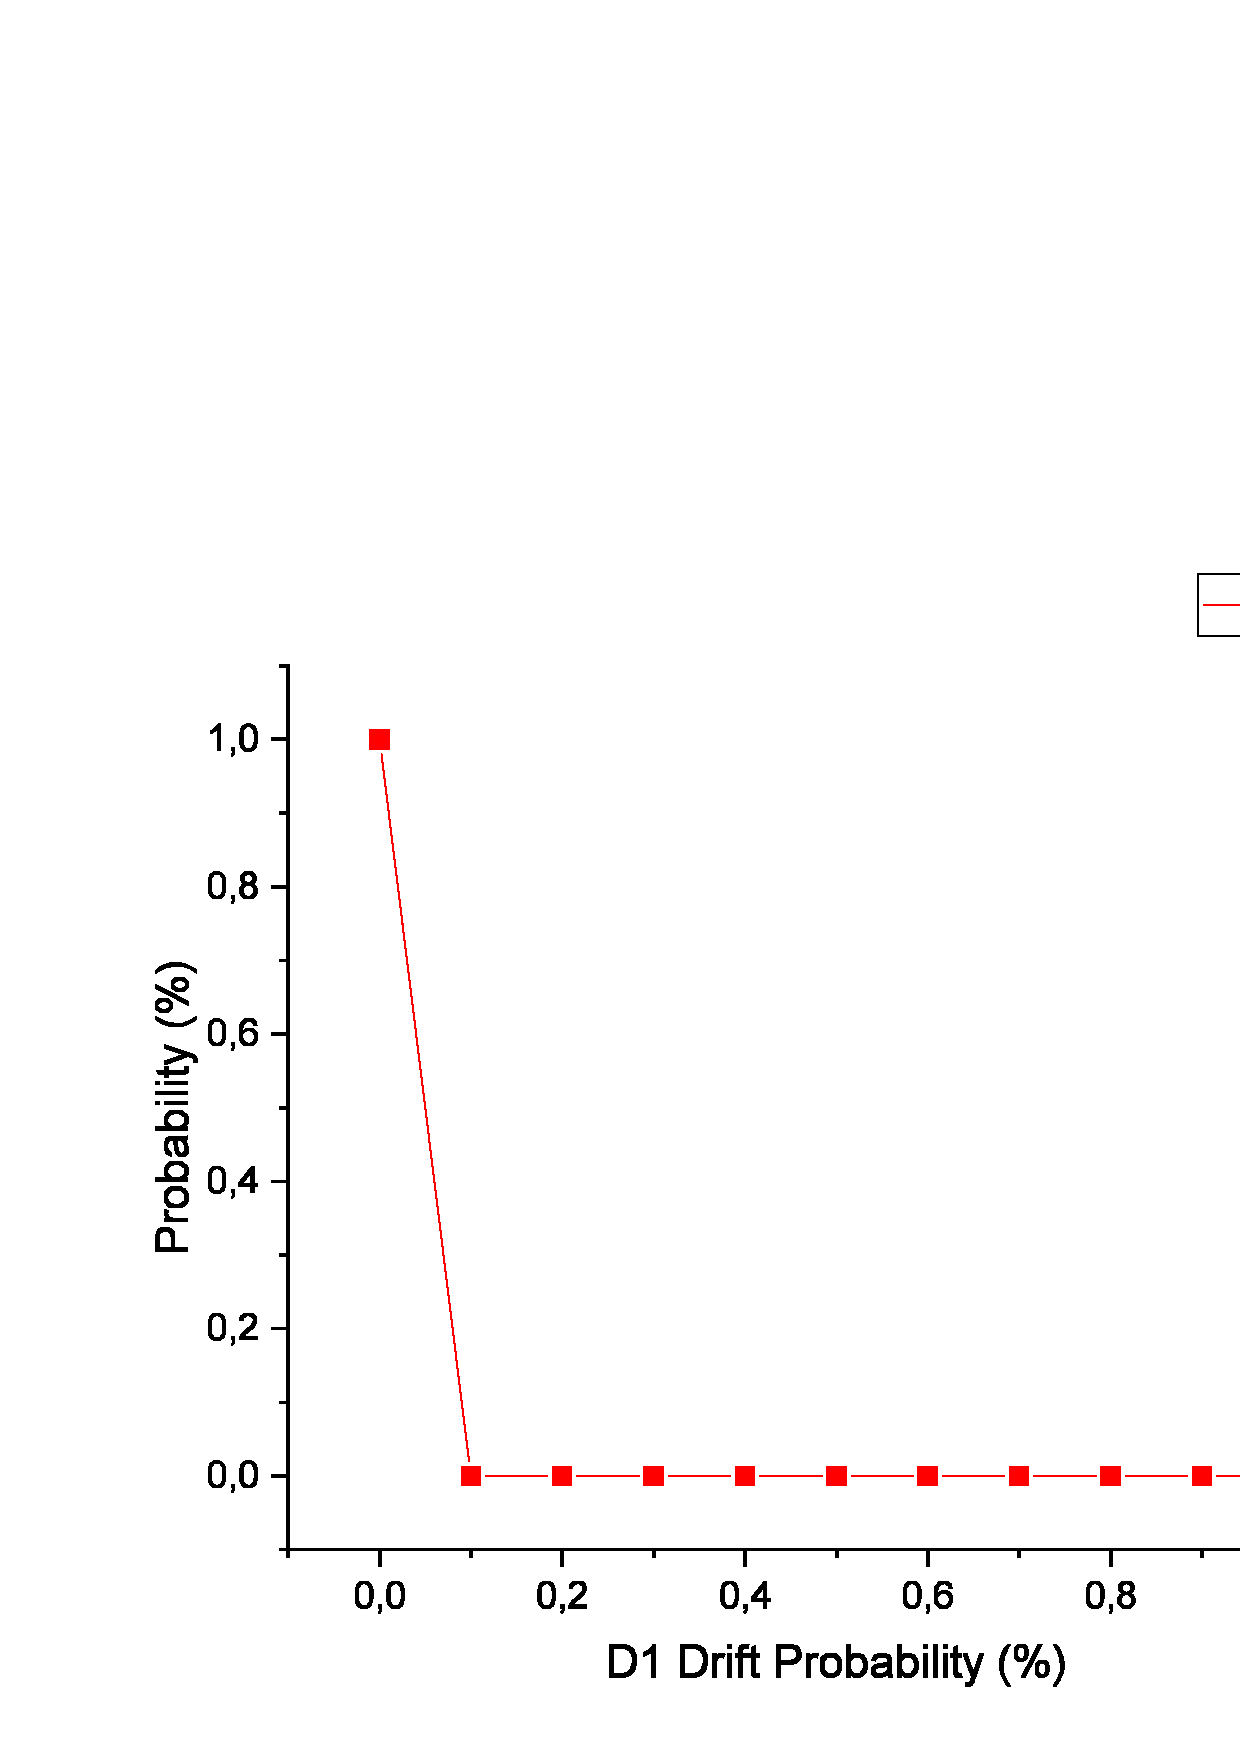
\includegraphics[width=200pt, height =110pt]{Graph2.pdf}
    \caption{Verification of Property \ref{eq2}.}
    \label{fig:02}
   \end{minipage}

       \\ 
    
           \end{tabularx}
\end{figure}

\noindent
    \begin{figure}[!htb]
       \begin{tabularx}{\linewidth}{ m{8cm}   m{8cm} }
           
%\noindent
 \begin{minipage}[t]{8cm}
     \centering

    \includegraphics[width=180pt, height =110pt]{Graph3.pdf}
    \caption{Verification of Property\ref{eq3}.}
    \label{fig:03}
   \end{minipage}
    
           &
%\noindent
   \begin{minipage}[t]{8cm}
     \centering
   		\includegraphics[width=200pt, height =110pt]{Graph4.pdf}
    \caption{Verification of Property \ref{eq2} for different time windows.}
    \label{fig:04}
   \end{minipage}

       \\ 
    
           \end{tabularx}
\end{figure}

The model is then verified against the previous properties in the context of DoS, MITM ARP spoofing, and Mirai attacks. We collect the rate of each attack to populate our CSG model. In the first case, we focus on attacks targeting the southbound bridge ports, which have an impact on the sensed data and corrupt its values (\emph{\bfseries{Property 1}}, \emph{\bfseries{Property 2}}). The second case investigates scenarios in which attacks have an impact on the routing keys (\emph{\bfseries{Property 3}}).

\subsubsection{On southbound bridges attacks}
For the first experiment, the label \quot{payload\_tamper}  in \emph{\bfseries{Property 1}} is implemented as the payload received at the southbound bridge differs from the expected attacker value. The model is downloadable from \cite{edcc23} with ID \quot{\texttt{M3}}. The results are portrayed in \fig{fig:01}. The player p1 represents the attacker, while p2 represents the sensors responsible for payload transmission. We observe that the payload tampering increases at each round of the CSG game to reach \emath{98\%}. However, the impacts of tampering differ from one attack to another, as it depends on the failure rate present in the dataset. During the experiment, it was observed that ARP spoofing had the highest impact on the model, followed by Mirai and DoS attacks.


The second experiment illustrates the damages incurred due to payload loss, as expressed in requirement \emph{\bfseries{Property 2}} using rPATL. The attacks do not exceed an acceptable increase of \emath{14\%} with respect to the sensitive infrastructure. However, to ensure accurate learning, the data must be correct and avoid the need for preprocessing. For example, in the research performed in \cite{Khalid2020}, a processing step involves removing outliers and erroneous data through mathematical operations, which is expensive regarding the large dataset. In \fig{fig:02}, The damage is primarily caused by ARP spoofing, followed by Mirai and DoS attacks, and remains stable at less than \emath{14\%}.

\subsubsection{On queues attacks}
The third experiment aims to investigate how the queue remains empty despite the payload messages being communicated to the gateway using property expressed in \emph{\bfseries{Property 3}}. The label \quot{empty} assigns a value of 0.5 (since there are two items in the queue), indicating that the queue is considered empty. Upon interpreting \fig{fig:03}, we observe that the queue is \emath{100\%} empty during the first five rounds, which is expected since the number of messages sent matches the total number of empty queues. However, we observe that the loss of payload messages is close to \emath{99\%} during the occurrence of tampering with the routing key. Other experiments could be conducted to investigate the impact of tampering with routing keys on the southbound bridges or the exchange module. However, since the results are expected to be similar to payload tampering, we have avoided performing these operations.

\subsection{Artefacts}
\label{sub:artefact}
The experiments elucidated in this section are openly accessible and entirely replicable. The source code can be obtained from the public GitHub website and repository \cite{edcc23}. The website offers comprehensive instructions on replicating the experiments and employing PRISM-games with individual examples. The repository encompasses a Python code that extracts the mean time between attacks from a CSV file to populate the PRISM model. The input dataset employed for learning is sourced from the Canadian Institute for Cybersecurity.

\section{Discussion}
\label{discussion}%\subsection{Risk Mitigation}
\subsection{Beyond model checking}
We have showcased the practicality of formal methods, particularly model checking of stochastic games with PRISM-games, in the modeling and verifying of the RabbitMQ communication \cmt{broker} for integration with the Sensinact gateway. We encoded the vital requirements of the RabbitMQ \cmt{broker} using rPATL and formally verified them. In the context of our experiment, these requirements encompassed the transmission of messages from sensors to the fog, ensuring that the messages are received even in the presence of DoS, Mirai, and ARP attacks that attempt to corrupt the payloads and the routing keys. In Section \ref{rabbitmq}, \cmt{we formalize rules about the occurrence of tampering during the transmission of payload messages and routing keys}. \cmt{Users may find implementing these rules in different formalisms beneficial instead of using the PRISM games language.} However, it should be noted that the verification process becomes lengthy when models incorporate a significant number of variables, such as queues with item variables. In our experiments, verifying the property in \emph{\bfseries{Property 3}} took 3 seconds to construct the model and 18 seconds to perform the verification. In such cases, abstraction could be beneficial in reducing the computational overhead.

\subsection{Risk mitigation}
Thanks to the Python artifacts we developed, we are able to capture the initial window of attacks and attempt to mitigate it by increasing the mean time between attacks. The mitigation strategy suggested by RabbitMQ in their documentation when an attack is detected is to ban the attacker for a specific duration, thereby extending the time window available for verification. The results of such modification are portrayed in \fig{fig:04} with PRISM code available on \cite{edcc23} with ID \quot{\texttt{M5}}. As the time window increases, the probability of message loss decreases, eventually reaching a low value of \emath{2\%}. This mitigation strategy demonstrates significant utility in scenarios where the system is comprehended and all potential environmental vulnerabilities are duly acknowledged.

\subsection{Network and latency}
\paragraph*{Networking using communication protocols} \cmt{RabbitMQ offers a wide range of communication mechanisms based on Bindings. These mechanisms allow for routing payload messages to specific queues or multiple queues. An efficient message broadcasting feature is provided through Fanout Exchanges, where messages are routed to all bound queues. This makes them particularly suitable for scenarios where the same information needs to be delivered to multiple consumers simultaneously. \cmt{Availability is enhanced through load balancing and message distribution by replicating data across queues}.
Additionally, RabbitMQ provides Remote Procedure Calls (RPC) \cite{rabbitmq-rpc} functionality. Implementing RPC over RabbitMQ is straightforward, as a client can send a request message and expect a response from the server. To ensure that the client receives the response, a 'callback' queue address must be included along with the request.} 


\paragraph*{Network Latency}  \cmt{The AMQP model of RabbitMQ includes queues, which can cause latency as their size grows. Moreover, RabbitMQ supports clustering and distribution, as described in the documentation \cite{rabbitmq-clustering}. Clustering ensures high availability by distributing message workloads across multiple nodes, enhancing overall reliability and performance even under network issues. Studied critical scenarios for performance evaluation are performed and explained in \cite{rabbitmq-performance}. We will delve deeper into the technical details of these clustering features in future work. }
\end{sloppypar}

\section{Related work}
\label{sec:rw}
\begin{sloppypar}
The literature review mentions a limited number of papers related to the formal verification of the RabbitMQ \cmt{broker}. However, it highlights the presence of research addressing validation through simulation. The RabbitMQ \cmt{broker} offers a range of robust features, including Authentication and Access Control \cite{rabbitmq-access-control}. This is achieved using JWT-encoded OAuth 2.0 access tokens \cite{rfc6749} and certificate-based client authentication. Another critical feature is Clustering, which ensures high availability and fault tolerance \cite{rabbitmq-clustering}. In the event of a node failure, clients can reconnect to an alternate node, recover their topology, and resume their operations uninterrupted. A wealth of related features can be found on the RabbitMQ documentation website \cite{rabbitmq-docs}. The RabbitMQ \cmt{broker} has undergone validation and verification in multiple studies, highlighting its distinguished features \cite{Li2020, Li2022, Ionescu2015, Hong2018, Bagaskara2020, Rostanski2014}.

The paper by  \citeauthor{Li2020} \cite{Li2020} presents a formal verification of the RabbitMQ \cmt{broker} using timed automata and the UPPAAL model checker\cite{behrmann2006uppaal}. Essential properties, including Reachability of Data and Message Acknowledgement, are successfully verified, confirming RabbitMQ's adherence to these properties. An extension of this work is presented in a subsequent article by \citeauthor{Li2022}  \cite{Li2022}, which emphasizes the integration of the Kerberos network authentication protocol \cite{Neuman1994}  to ensure secure communication (related to authentication). Using UPPAAL \cite{behrmann2006uppaal}, the authors model and verify the enhanced protocol, providing evidence of RabbitMQ's ability to maintain secure communication.

In the paper by \citeauthor{Ionescu2015} \cite{Ionescu2015}, a performance comparison of RabbitMQ and ActiveMQ \cite{activemq} brokers in message-oriented middleware applications is conducted, with a specific focus on message sending and receiving. The analysis reveals distinctions between the two brokers: ActiveMQ exhibits superior message reception speed, while RabbitMQ demonstrates qualitative message delivery to clients due to its implemented security functions during reception. Furthermore, \citeauthor{Rostanski2014} \cite{Rostanski2014}  investigate design considerations for scalability and high availability in RabbitMQ. The study explores the usage of clustered RabbitMQ nodes and mirrored queues and presents simulation test results to evaluate performance.

During our review of the relevant literature, we came across the work conducted by \citeauthor{Li2020} \cite{Li2020}, which primarily focuses on the functional properties of RabbitMQ using UPPAAL. An extension of their work is presented in \citeauthor{Li2022}  \cite{Li2022}, where they specifically address verification of unauthorized access to the communication channel. In contrast, studies such as \cite{Ionescu2015, Hong2018, Bagaskara2020, Rostanski2014} primarily utilize simulation techniques to assess performance aspects of deployed servers, including scalability, memory usage, and throughput. However, these studies do not consider the security aspects related to unauthorized data modification given the complexity of the architecture. In contrast, our paper aims to bridge this gap by providing a comprehensive approach to modeling and analyzing unauthorized data modification attacks within the considered system architecture. We accomplish this by employing a game model that captures concurrent access through Concurrent Stochastic Games (CSGs) using the PRISM games.


\cmt{We rely on a straightforward algorithm that utilizes Python libraries when extracting attack frequency and optimizing techniques. This algorithm allows us to calculate the Mean Time Between Attacks (MTBA) from the dataset using established algorithms from the literature, such as the Broyden–Fletcher–Goldfarb–Shanno algorithm (L-BFGS-B) \cite{liu1989limited} and the Nelder-Mead algorithm \cite{nelder1965simplex}. These algorithms have been widely used in the field and are known for their effectiveness in this context. Other nature-inspired metaheuristic algorithm, specifically focusing on optimization techniques that could be used in such optimization.  In \citeauthor{Genghis2023} in \cite{Genghis2023} introduces a nature-inspired metaheuristic algorithm called GKS optimizer (GKSO), inspired by the behavior of the Genghis Khan shark. GKSO  performs optimization tasks achieved by simulating hunting, movement, foraging, and self-protection mechanisms. The algorithm's viability and superiority are validated through qualitative and quantitative analyses, demonstrating its exploration and exploitation capabilities. \citeauthor{Ezugwu2022} in  \cite{Ezugwu2022} introduces prairie dog optimization (PDO), a nature-inspired metaheuristic algorithm that mimics the behavior of prairie dogs in their natural habitat. PDO utilizes foraging and burrow-build activities for exploration while exploiting the prairie dogs' communication skills to converge toward promising locations. \citeauthor{Jeffrey2022} in  \cite{Jeffrey2022} presents the dwarf mongoose optimization (DMO) algorithm inspired by the foraging behavior of dwarf mongooses. DMO utilizes three social groups (alpha group, babysitters, and scout group) to mimic the mongoose's foraging strategy. \citeauthor{Agushaka2023} in  \cite{Agushaka2023} introduces the Gazelle Optimization Algorithm (GOA), inspired by the survival behavior of gazelles in predator-dominated environments. The algorithm incorporates two phases: exploitation, where gazelles graze peacefully, and exploration, evading predators.} 

\cmt{\citeauthor{DETDO2023} in \cite{DETDO2023} presents DETDO, an adaptive hybrid dandelion optimizer based on the Dandelion Optimizer (DO). DETDO combines adaptive tent chaotic mapping, differential evolution strategy, and adaptive t-distribution perturbation to prevent local optima and improve convergence speed. \citeauthor{Mojtaba2024} in \cite{Mojtaba2024} introduces Lung performance-based optimization (LPO) inspired by the performance of lungs in the human body. LPO draws inspiration from the adaptability and optimization of the respiratory system in solving complex optimization problems.}
\end{sloppypar}

\section{Conclusion}\label{conclusion}
\begin{sloppypar}
This paper investigates the impact of clock deviation within a component-port-connector architecture model. The OMNeT++ framework defines the behavior of system components and connectors. The resulting model is then translated into the PRISM language, utilizing Probabilistic Decision Tree rules derived from the OMNeT++ simulation trace. Requirements related to synchronized clocks, expressed in Probabilistic Computation Tree Logic (PCTL), are verified against two models constructed in PRISM \cmt{PA}: a reference model and one generated by learning decision trees. A use case is then implemented in both formalisms to demonstrate the effectiveness of the proposed approach for validation. 

The models incorporate parameters inspired by real-world phenomena observed in standard specifications, including product manufacturing variations and operating temperature changes. This parameterized construction allows practitioners to perform customized validation and verification. Our results demonstrate that building stochastic models from simulated models leads to more efficient models with fewer states and transitions compared to PRISM models.

In future research endeavors, we plan to formally capture the bi-simulation between the constructed models and the learned abstract model. This task presents a significant challenge due to the potential differences in the state spaces of the input and abstract models. Additionally, we aim to develop an automated approach for feature selection during the learning process. The current approach, while promising, requires human intervention in choosing the features used for model construction. \cmt{Finally, to enhance realism, we plan to incorporate more precise communication delays. We aim to achieve this by utilizing electronic tools for delay measurement or more advanced simulation techniques.}
\end{sloppypar}



\subsection*{Acknowledgement}
The research leading to the presented results was conducted within the research profile of \acisiot (ACIS-IoT), supported by the Centre National de la Recherche Scientifique (CNRS). The authors express their gratitude to the individuals involved in the European projects CPS4EU and BRAIN-IoT projects, acknowledging their valuable contributions and feedback.



%\bibliographystyle{model1a-num-names}
%\bibliographystyle{plainnat}
%\bibliographystyle{model3-num-names}

\bibliographystyle{elsarticle-num-names}
\bibliography{references}


\end{document}
